% Options for packages loaded elsewhere
\PassOptionsToPackage{unicode}{hyperref}
\PassOptionsToPackage{hyphens}{url}
%
\documentclass[
]{article}
\usepackage{amsmath,amssymb}
\usepackage{iftex}
\ifPDFTeX
  \usepackage[T1]{fontenc}
  \usepackage[utf8]{inputenc}
  \usepackage{textcomp} % provide euro and other symbols
\else % if luatex or xetex
  \usepackage{unicode-math} % this also loads fontspec
  \defaultfontfeatures{Scale=MatchLowercase}
  \defaultfontfeatures[\rmfamily]{Ligatures=TeX,Scale=1}
\fi
\usepackage{lmodern}
\ifPDFTeX\else
  % xetex/luatex font selection
\fi
% Use upquote if available, for straight quotes in verbatim environments
\IfFileExists{upquote.sty}{\usepackage{upquote}}{}
\IfFileExists{microtype.sty}{% use microtype if available
  \usepackage[]{microtype}
  \UseMicrotypeSet[protrusion]{basicmath} % disable protrusion for tt fonts
}{}
\makeatletter
\@ifundefined{KOMAClassName}{% if non-KOMA class
  \IfFileExists{parskip.sty}{%
    \usepackage{parskip}
  }{% else
    \setlength{\parindent}{0pt}
    \setlength{\parskip}{6pt plus 2pt minus 1pt}}
}{% if KOMA class
  \KOMAoptions{parskip=half}}
\makeatother
\usepackage{xcolor}
\usepackage[margin=1in]{geometry}
\usepackage{longtable,booktabs,array}
\usepackage{calc} % for calculating minipage widths
% Correct order of tables after \paragraph or \subparagraph
\usepackage{etoolbox}
\makeatletter
\patchcmd\longtable{\par}{\if@noskipsec\mbox{}\fi\par}{}{}
\makeatother
% Allow footnotes in longtable head/foot
\IfFileExists{footnotehyper.sty}{\usepackage{footnotehyper}}{\usepackage{footnote}}
\makesavenoteenv{longtable}
\usepackage{graphicx}
\makeatletter
\def\maxwidth{\ifdim\Gin@nat@width>\linewidth\linewidth\else\Gin@nat@width\fi}
\def\maxheight{\ifdim\Gin@nat@height>\textheight\textheight\else\Gin@nat@height\fi}
\makeatother
% Scale images if necessary, so that they will not overflow the page
% margins by default, and it is still possible to overwrite the defaults
% using explicit options in \includegraphics[width, height, ...]{}
\setkeys{Gin}{width=\maxwidth,height=\maxheight,keepaspectratio}
% Set default figure placement to htbp
\makeatletter
\def\fps@figure{htbp}
\makeatother
\setlength{\emergencystretch}{3em} % prevent overfull lines
\providecommand{\tightlist}{%
  \setlength{\itemsep}{0pt}\setlength{\parskip}{0pt}}
\setcounter{secnumdepth}{-\maxdimen} % remove section numbering
\usepackage{float}
\ifLuaTeX
  \usepackage{selnolig}  % disable illegal ligatures
\fi
\usepackage{bookmark}
\IfFileExists{xurl.sty}{\usepackage{xurl}}{} % add URL line breaks if available
\urlstyle{same}
\hypersetup{
  pdftitle={Imputation Analysis Report},
  hidelinks,
  pdfcreator={LaTeX via pandoc}}

\title{Imputation Analysis Report}
\author{}
\date{\vspace{-2.5em}}

\begin{document}
\maketitle

\section{Dataset Information}\label{dataset-information}

\textbf{Data file used:} blood\_storage\_example\\
\textbf{Overall missing rate:} 15.54\%

\textbf{Variables used for imputation:}

\begin{itemize}
\tightlist
\item
  Median.RBC.Age\\
\item
  Age\\
\item
  PVol\\
\item
  PreopPSA\\
\item
  Units\\
\item
  TimeToRecurrence\\
\item
  RBC.Age.Group\\
\item
  TVol\\
\item
  T.Stage\\
\item
  bGS\\
\item
  sGS\\
\item
  AA\\
\item
  FamHx\\
\item
  BN+\\
\item
  OrganConfined\\
\item
  PreopTherapy\\
\item
  AnyAdjTherapy\\
\item
  AdjRadTherapy\\
\item
  Recurrence\\
\item
  Censor
\end{itemize}

\textbf{Best model selected: }RandomForest\\
\textbf{Imputed dataset saved as: }final\_imputed\_data\_rf.csv

\section{Correlation Heatmaps}\label{correlation-heatmaps}

\begin{figure}[H]

{\centering 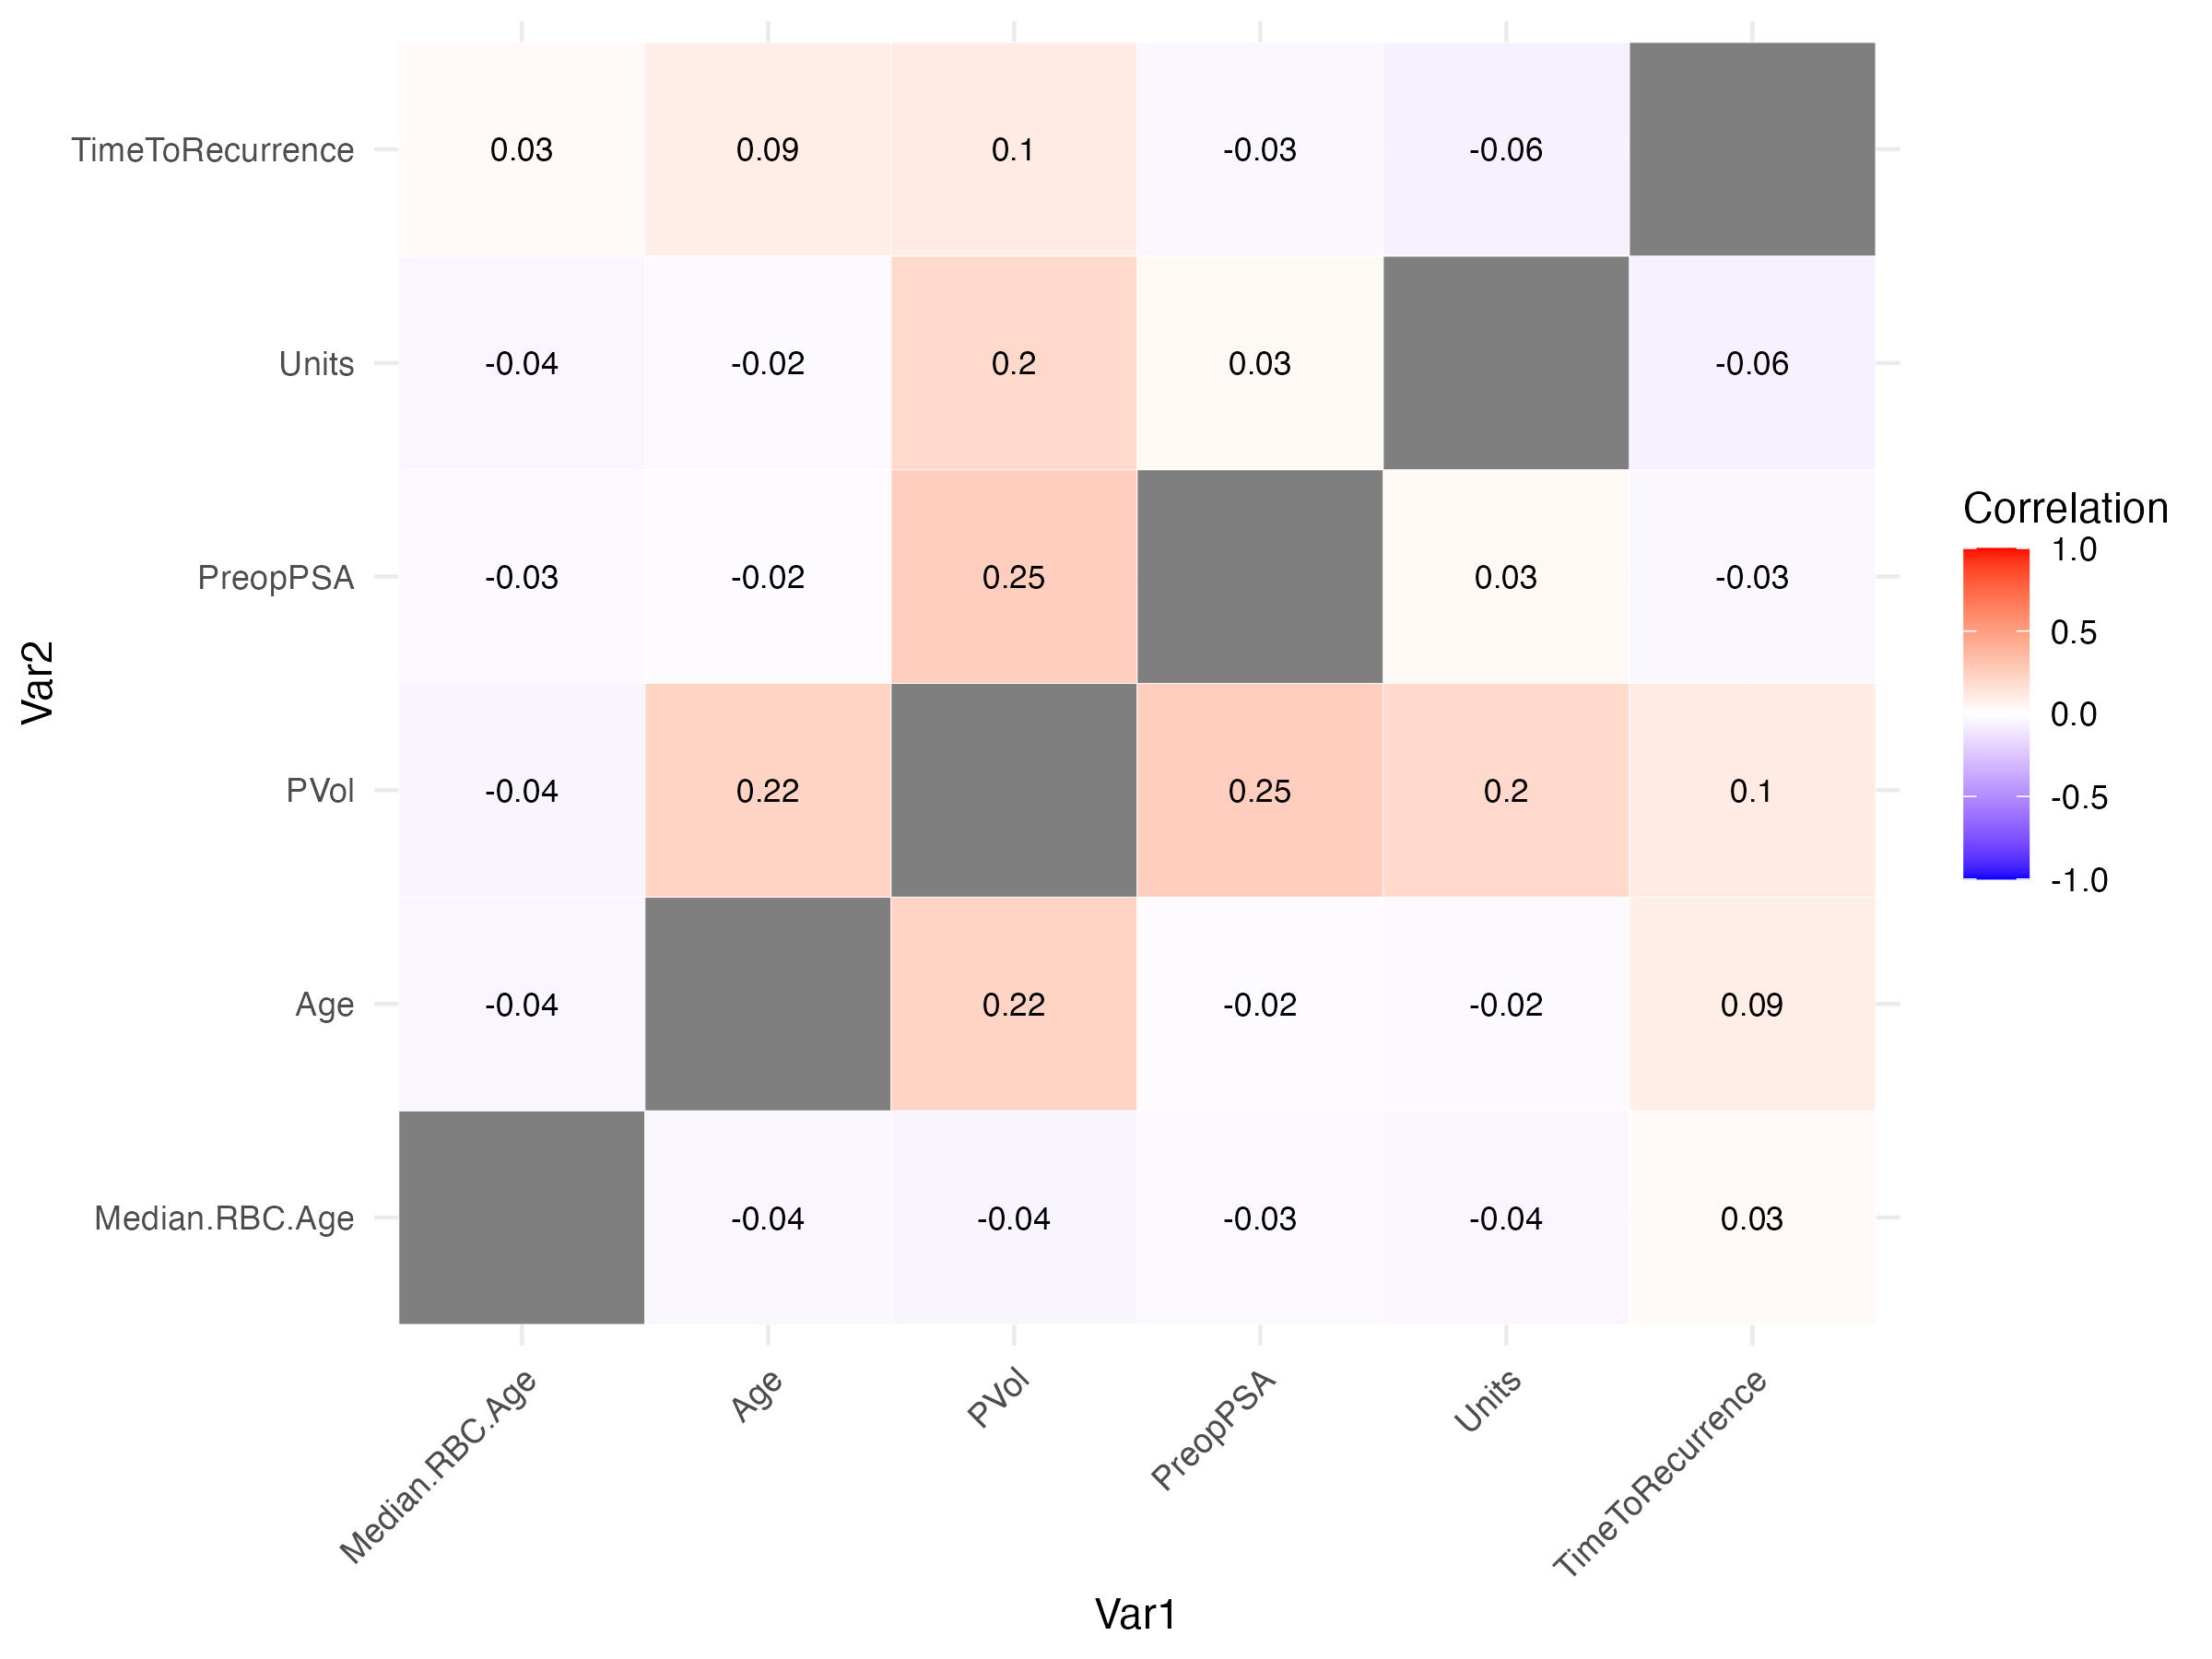
\includegraphics[width=0.9\linewidth]{../example/correlation_heatmap_continuous} 

}

\caption{Correlation Heatmap - Continuous Variables}\label{fig:show-cor-cont}
\end{figure}

\begin{figure}[H]

{\centering 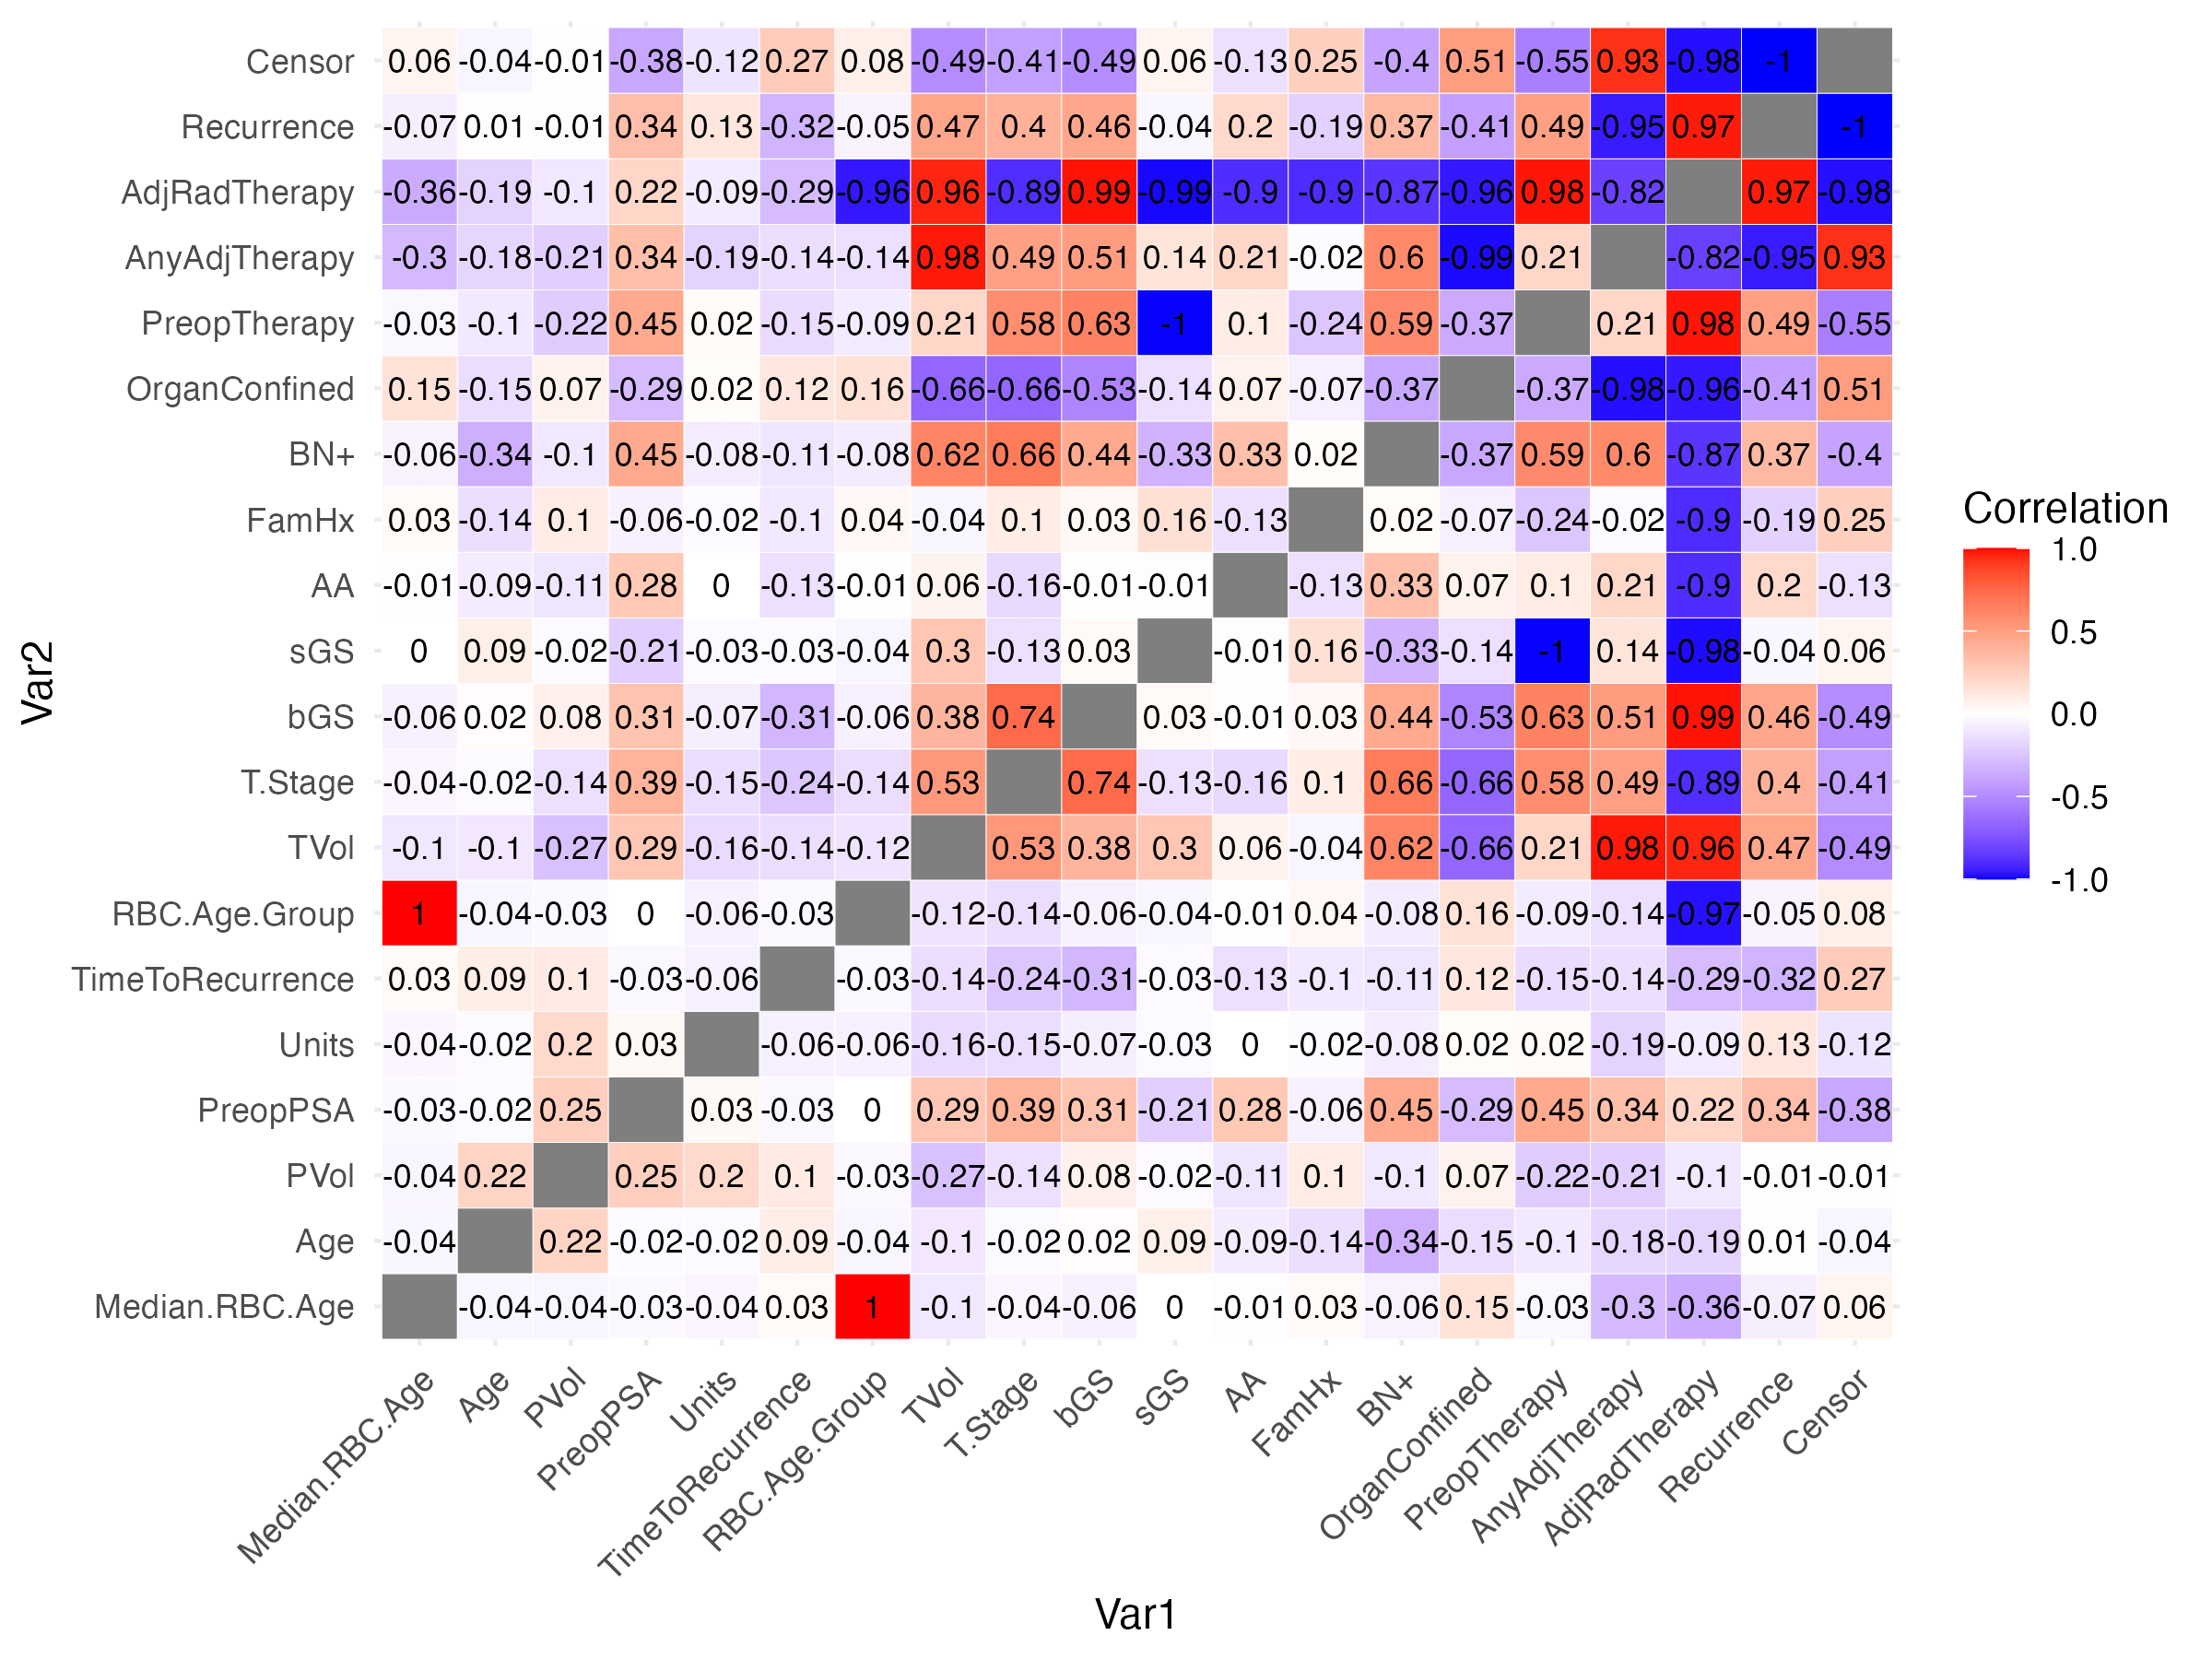
\includegraphics[width=0.9\linewidth]{../example/correlation_heatmap_all} 

}

\caption{Correlation Heatmap - All Variables}\label{fig:show-cor-all}
\end{figure}

\section{Imputation Settings}\label{imputation-settings}

\textbf{Imputation Configuration:}\\
- Missing rate levels (\texttt{list\_noNA}): 0.05, 0.1, 0.15, 0.2\\
- Number of Trees (\texttt{ntree}): 50\\
- Maximum Number of Iterations in RandomForest (\texttt{maxiter}): 5\\
- K values for KNN (\texttt{k\_values}): 3, 5, 7\\
- MICE iterations (\texttt{mice\_m}): 3\\
- MICE maxit (\texttt{mice\_maxit}): 5\\
- Number of decision trees in MiceRanger (\texttt{micer\_num\_trees}):
50\\
- Random seed (\texttt{seed}): 123\\
- Number of iterations (\texttt{niter}): 2\\
- Methods used to simulate imputation (\texttt{methods}): rf, mice

\newpage

\section{Model Performance Summary}\label{model-performance-summary}

\begin{longtable}[]{@{}
  >{\raggedright\arraybackslash}p{(\columnwidth - 8\tabcolsep) * \real{0.1912}}
  >{\raggedleft\arraybackslash}p{(\columnwidth - 8\tabcolsep) * \real{0.1912}}
  >{\raggedleft\arraybackslash}p{(\columnwidth - 8\tabcolsep) * \real{0.1765}}
  >{\raggedleft\arraybackslash}p{(\columnwidth - 8\tabcolsep) * \real{0.2500}}
  >{\raggedright\arraybackslash}p{(\columnwidth - 8\tabcolsep) * \real{0.1912}}@{}}
\caption{Model Performance Across Missing Rates}\tabularnewline
\toprule\noalign{}
\begin{minipage}[b]{\linewidth}\raggedright
Method
\end{minipage} & \begin{minipage}[b]{\linewidth}\raggedleft
Missing\_Rate
\end{minipage} & \begin{minipage}[b]{\linewidth}\raggedleft
Average\_MSE
\end{minipage} & \begin{minipage}[b]{\linewidth}\raggedleft
Average\_Accuracy
\end{minipage} & \begin{minipage}[b]{\linewidth}\raggedright
Best\_K\_Value
\end{minipage} \\
\midrule\noalign{}
\endfirsthead
\toprule\noalign{}
\begin{minipage}[b]{\linewidth}\raggedright
Method
\end{minipage} & \begin{minipage}[b]{\linewidth}\raggedleft
Missing\_Rate
\end{minipage} & \begin{minipage}[b]{\linewidth}\raggedleft
Average\_MSE
\end{minipage} & \begin{minipage}[b]{\linewidth}\raggedleft
Average\_Accuracy
\end{minipage} & \begin{minipage}[b]{\linewidth}\raggedright
Best\_K\_Value
\end{minipage} \\
\midrule\noalign{}
\endhead
\bottomrule\noalign{}
\endlastfoot
MICE & 0.05 & 0.0928285 & 0.9873810 & NA \\
RandomForest & 0.05 & 0.0251190 & 0.9935714 & NA \\
MICE & 0.10 & 0.1780190 & 0.9750000 & NA \\
RandomForest & 0.10 & 0.1133017 & 0.9845238 & NA \\
MICE & 0.15 & 0.1727021 & 0.9540476 & NA \\
RandomForest & 0.15 & 0.1167390 & 0.9726190 & NA \\
MICE & 0.20 & 0.2953958 & 0.9419048 & NA \\
RandomForest & 0.20 & 0.1684802 & 0.9642857 & NA \\
\end{longtable}

\begin{figure}[H]

{\centering 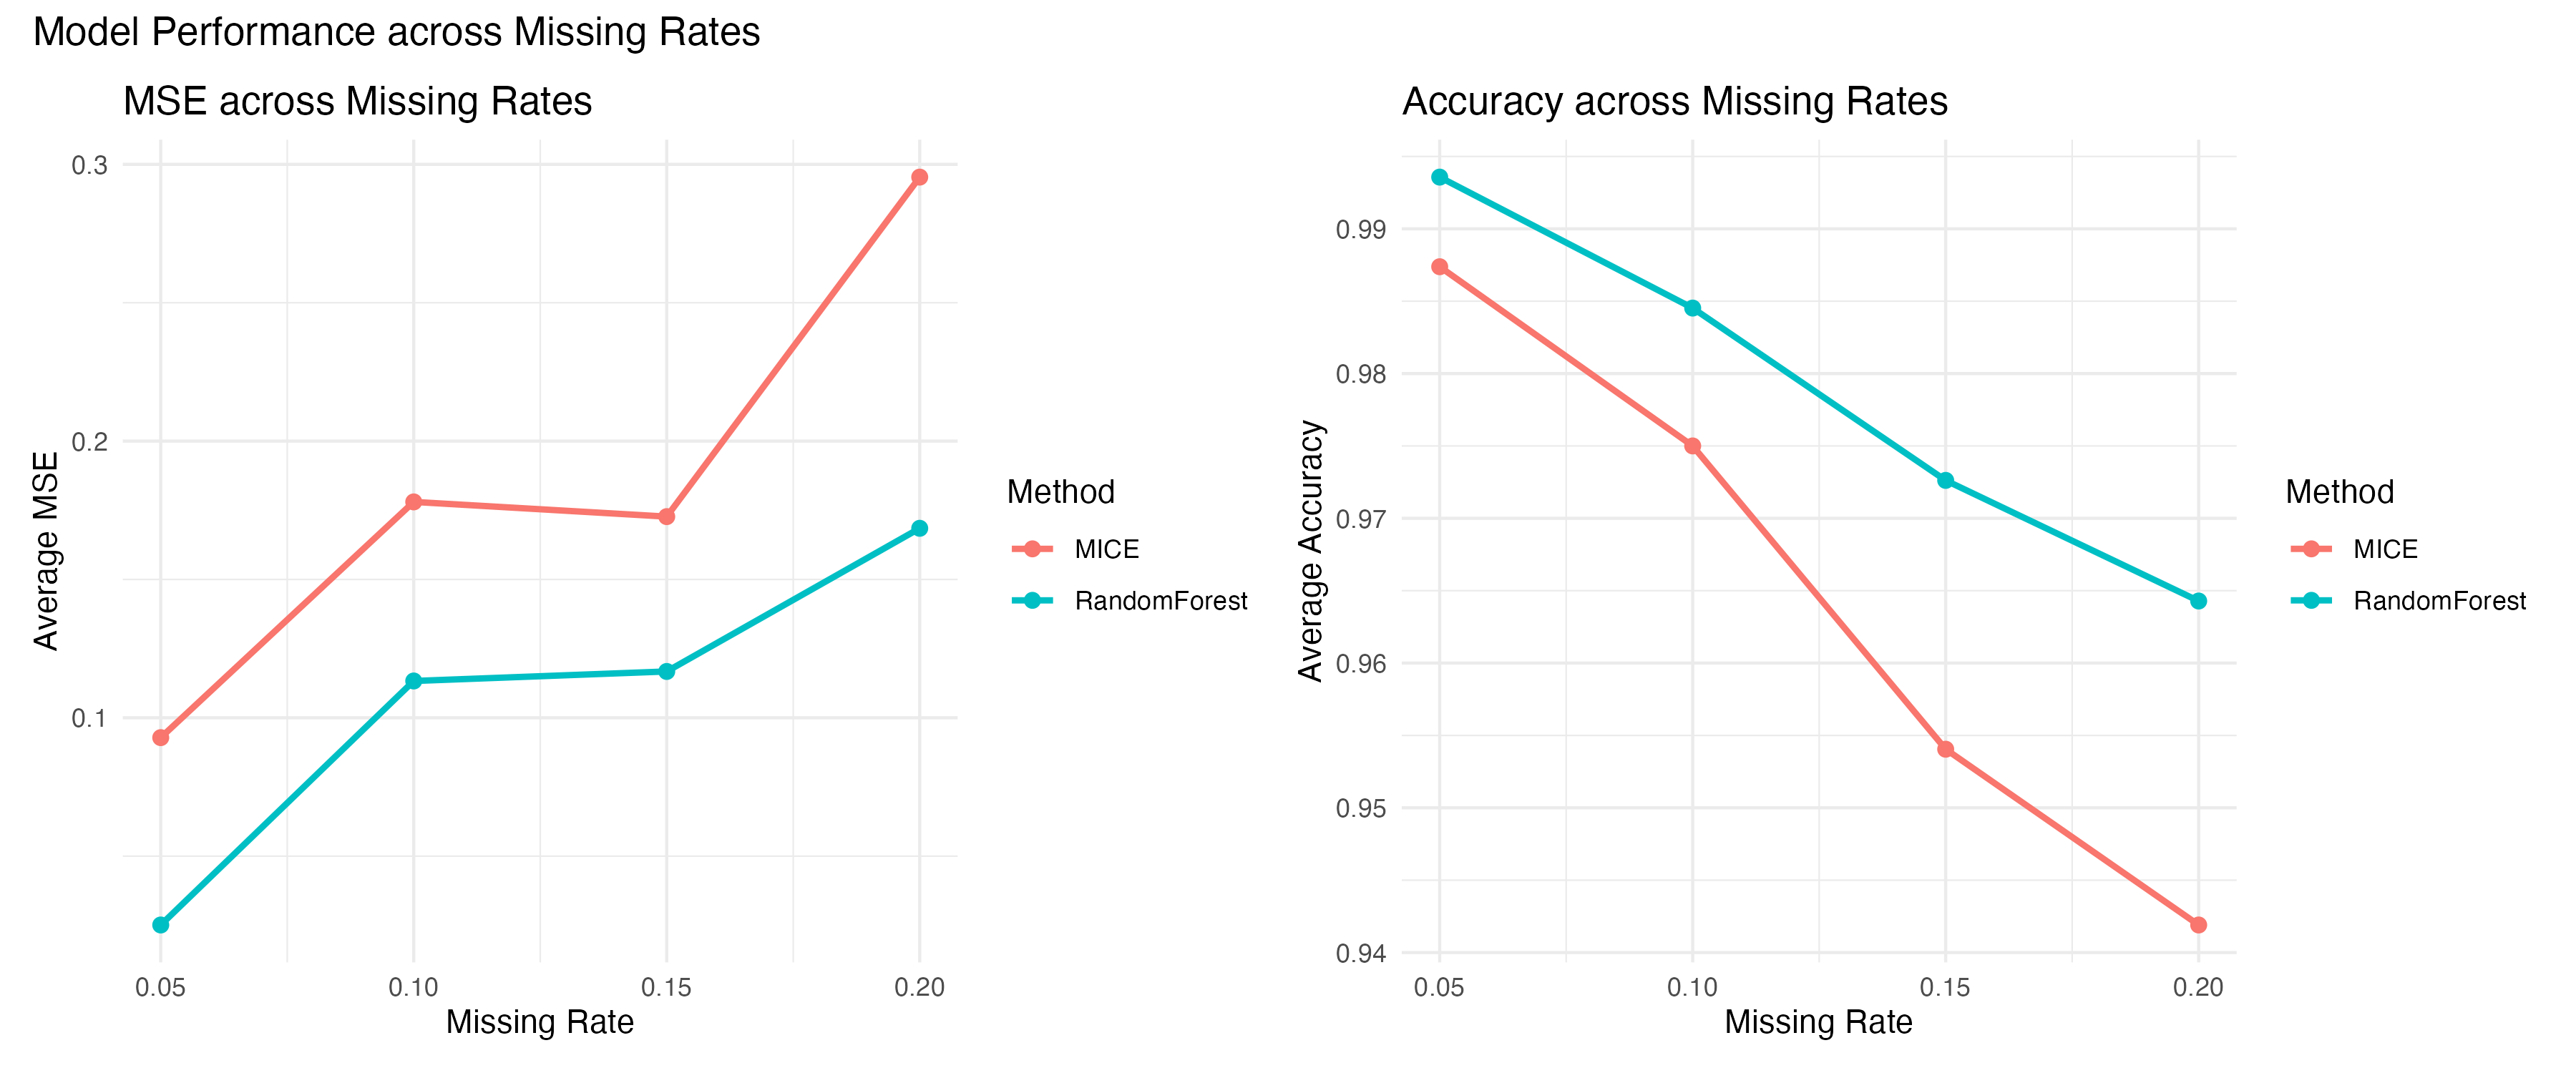
\includegraphics[width=0.9\linewidth]{../example/lineplot_MSE_Accuracy_combined} 

}

\caption{Performance Performance Comparison Plot Across Missing Rates}\label{fig:show-performance-lineplot}
\end{figure}

\section{Imputation Comparison: Before vs
After}\label{imputation-comparison-before-vs-after}

\begin{longtable}[]{@{}lrr@{}}
\caption{Missing Values Before vs.~After Imputation}\tabularnewline
\toprule\noalign{}
Variable & Missing\_Before & Missing\_After \\
\midrule\noalign{}
\endfirsthead
\toprule\noalign{}
Variable & Missing\_Before & Missing\_After \\
\midrule\noalign{}
\endhead
\bottomrule\noalign{}
\endlastfoot
Median.RBC.Age & 43 & 0 \\
Age & 49 & 0 \\
PVol & 55 & 0 \\
PreopPSA & 45 & 0 \\
Units & 43 & 0 \\
TimeToRecurrence & 50 & 0 \\
RBC.Age.Group & 49 & 0 \\
TVol & 60 & 0 \\
T.Stage & 54 & 0 \\
bGS & 49 & 0 \\
sGS & 51 & 0 \\
AA & 47 & 0 \\
FamHx & 43 & 0 \\
BN+ & 50 & 0 \\
OrganConfined & 50 & 0 \\
PreopTherapy & 50 & 0 \\
AnyAdjTherapy & 43 & 0 \\
AdjRadTherapy & 43 & 0 \\
Recurrence & 54 & 0 \\
Censor & 54 & 0 \\
\end{longtable}

\begin{longtable}[t]{lrr}
\caption{\label{tab:compare-before-after}Summary Statistics Before vs. After Imputation}\\
\toprule
Variable\_Statistic & Before & After\\
\midrule
Median.RBC.Age\_mean & 16.648352 & 17.089385\\
Median.RBC.Age\_sd & 6.259769 & 6.210462\\
Median.RBC.Age\_min & 10.000000 & 10.000000\\
Median.RBC.Age\_max & 25.000000 & 25.000000\\
Age\_mean & 61.124345 & 61.219344\\
\addlinespace
Age\_sd & 7.208566 & 6.715862\\
Age\_min & 38.400000 & 38.400000\\
Age\_max & 79.000000 & 79.000000\\
PVol\_mean & 56.052874 & 56.575945\\
PVol\_sd & 31.260544 & 28.786488\\
\addlinespace
PVol\_min & 19.400000 & 19.400000\\
PVol\_max & 274.000000 & 274.000000\\
PreopPSA\_mean & 8.216052 & 8.167973\\
PreopPSA\_sd & 6.011284 & 5.659542\\
PreopPSA\_min & 1.300000 & 1.300000\\
\addlinespace
PreopPSA\_max & 39.000000 & 39.000000\\
Units\_mean & 2.454213 & 2.446114\\
Units\_sd & 1.832787 & 1.712699\\
Units\_min & 1.000000 & 1.000000\\
Units\_max & 19.000000 & 19.000000\\
\addlinespace
TimeToRecurrence\_mean & 32.500489 & 33.122535\\
TimeToRecurrence\_sd & 28.111005 & 26.241702\\
TimeToRecurrence\_min & 0.270000 & 0.270000\\
TimeToRecurrence\_max & 103.600000 & 103.600000\\
\bottomrule
\end{longtable}

\begin{figure}[H]

{\centering 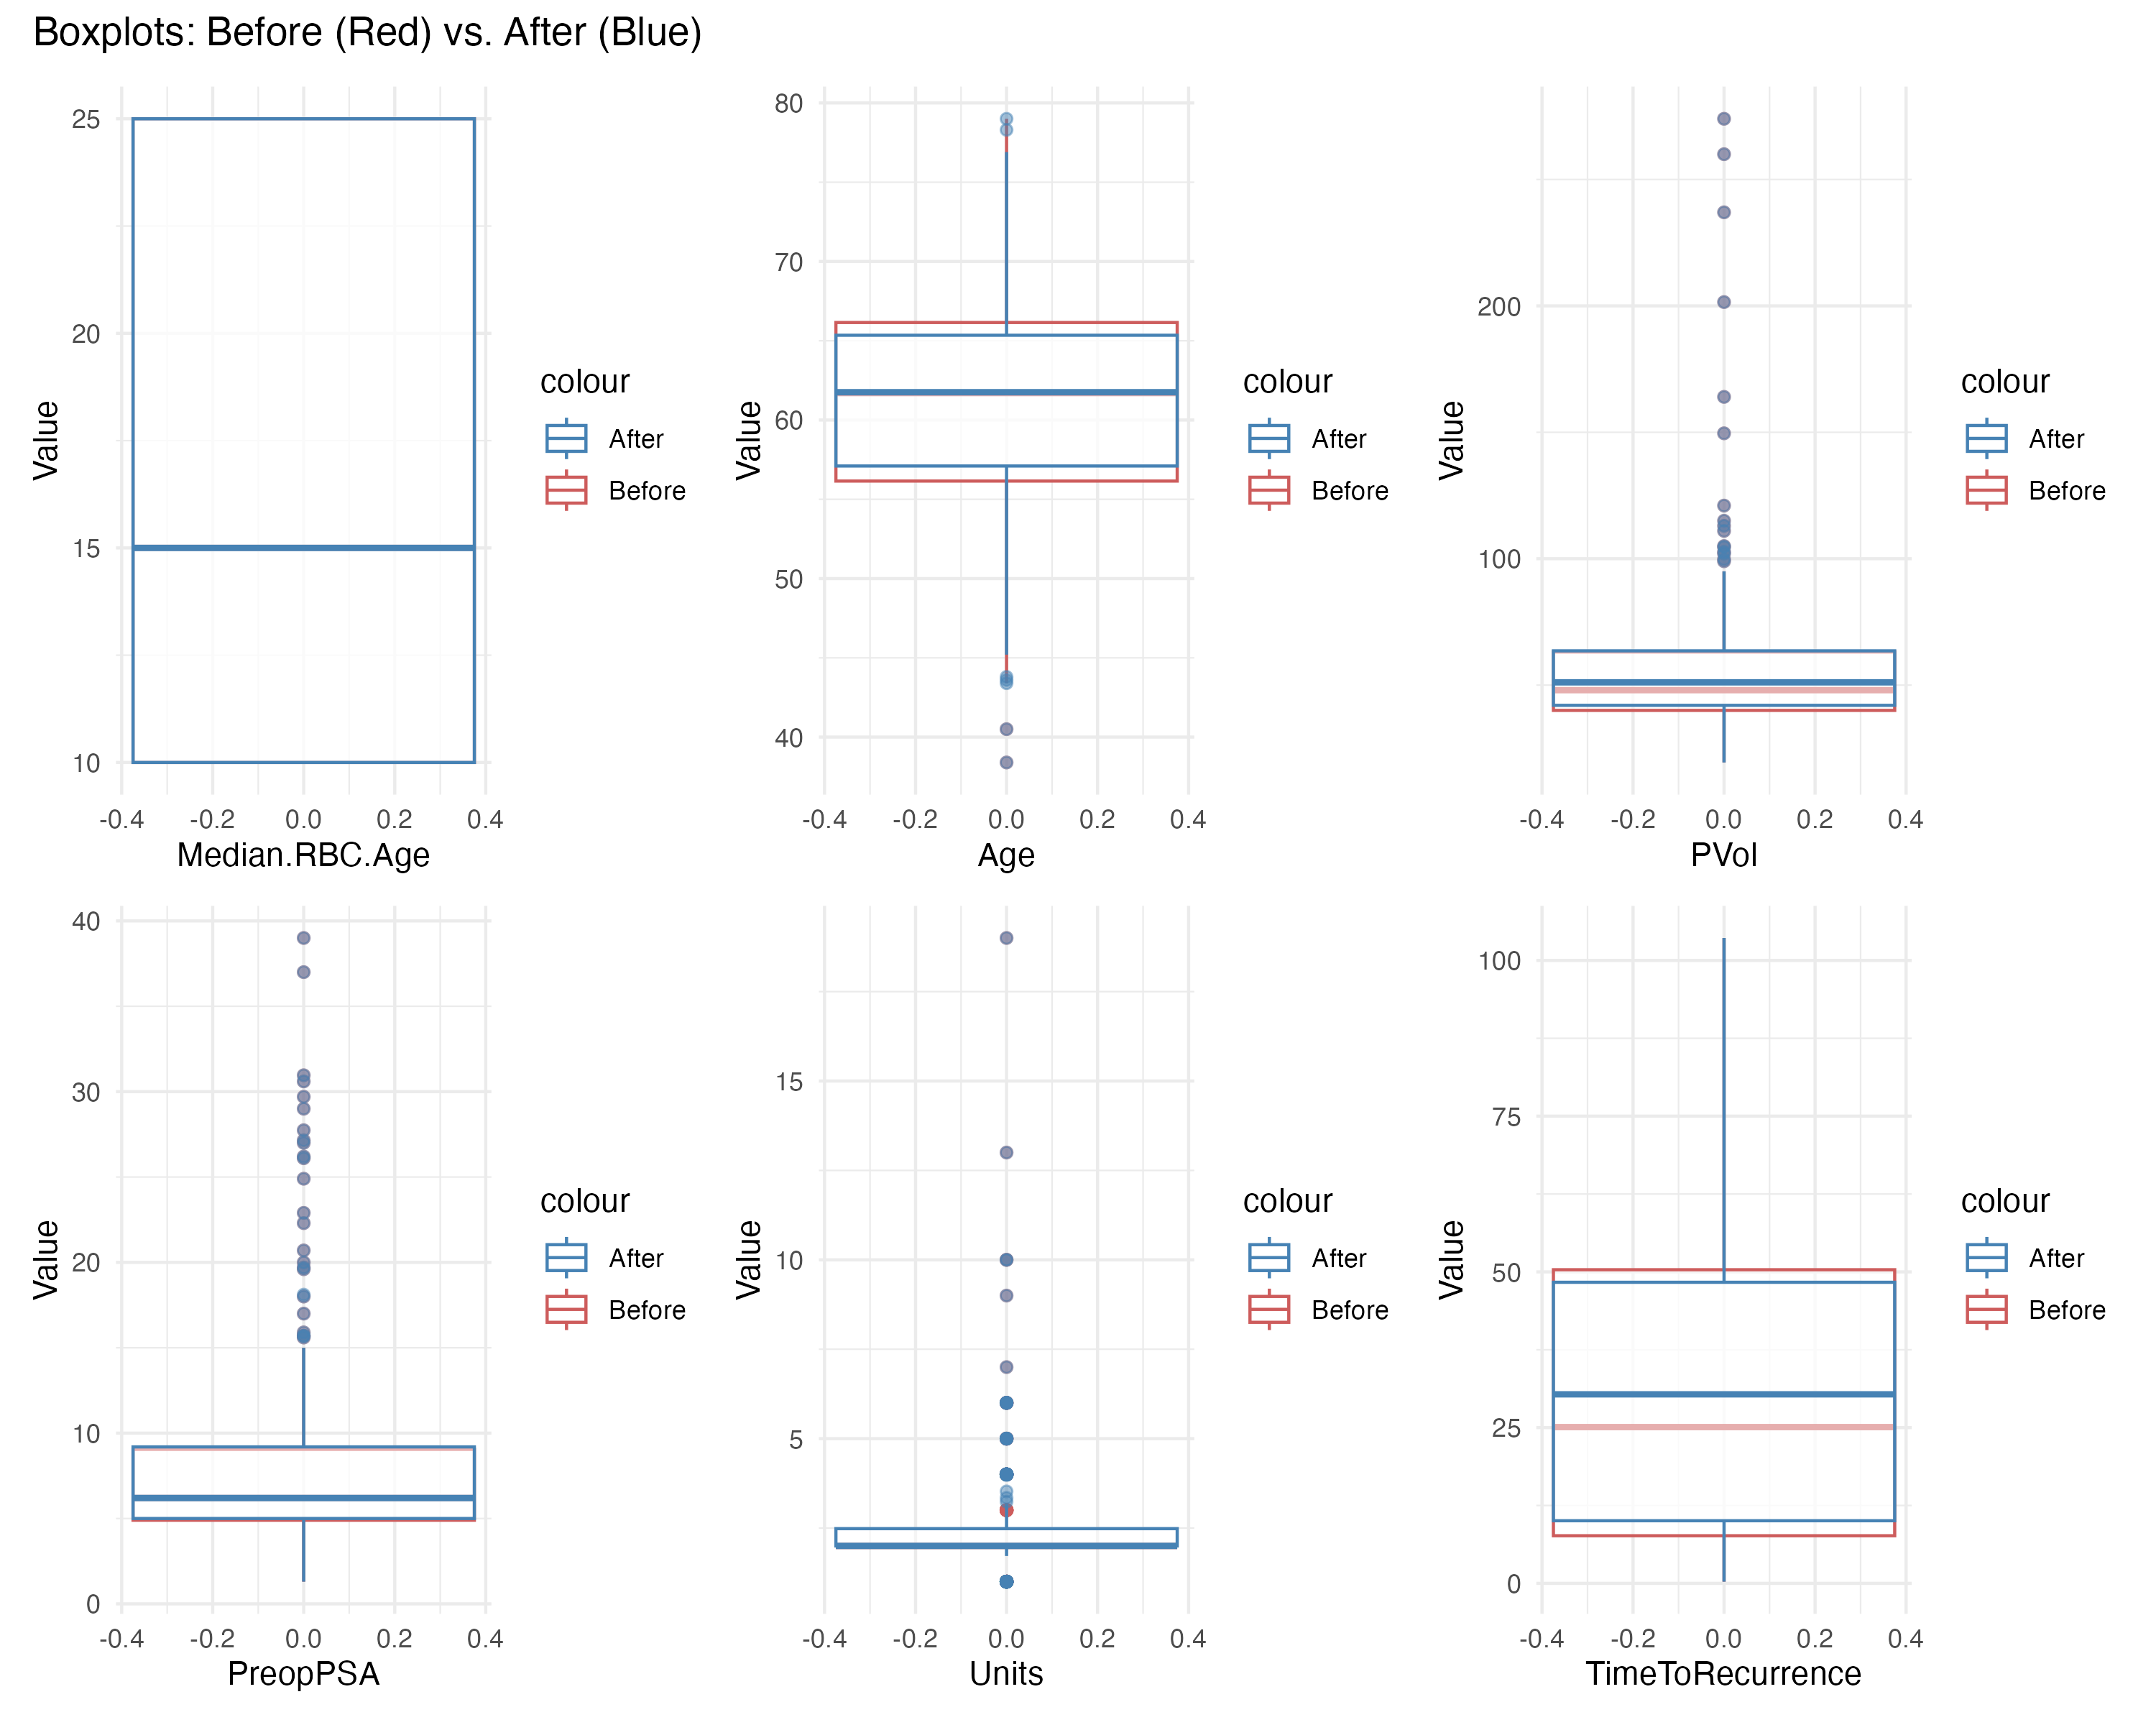
\includegraphics[width=0.9\linewidth]{../example/boxplots_before_after} 

}

\caption{Boxplots (Before vs After)}\label{fig:show-boxplot}
\end{figure}

\begin{figure}[H]

{\centering 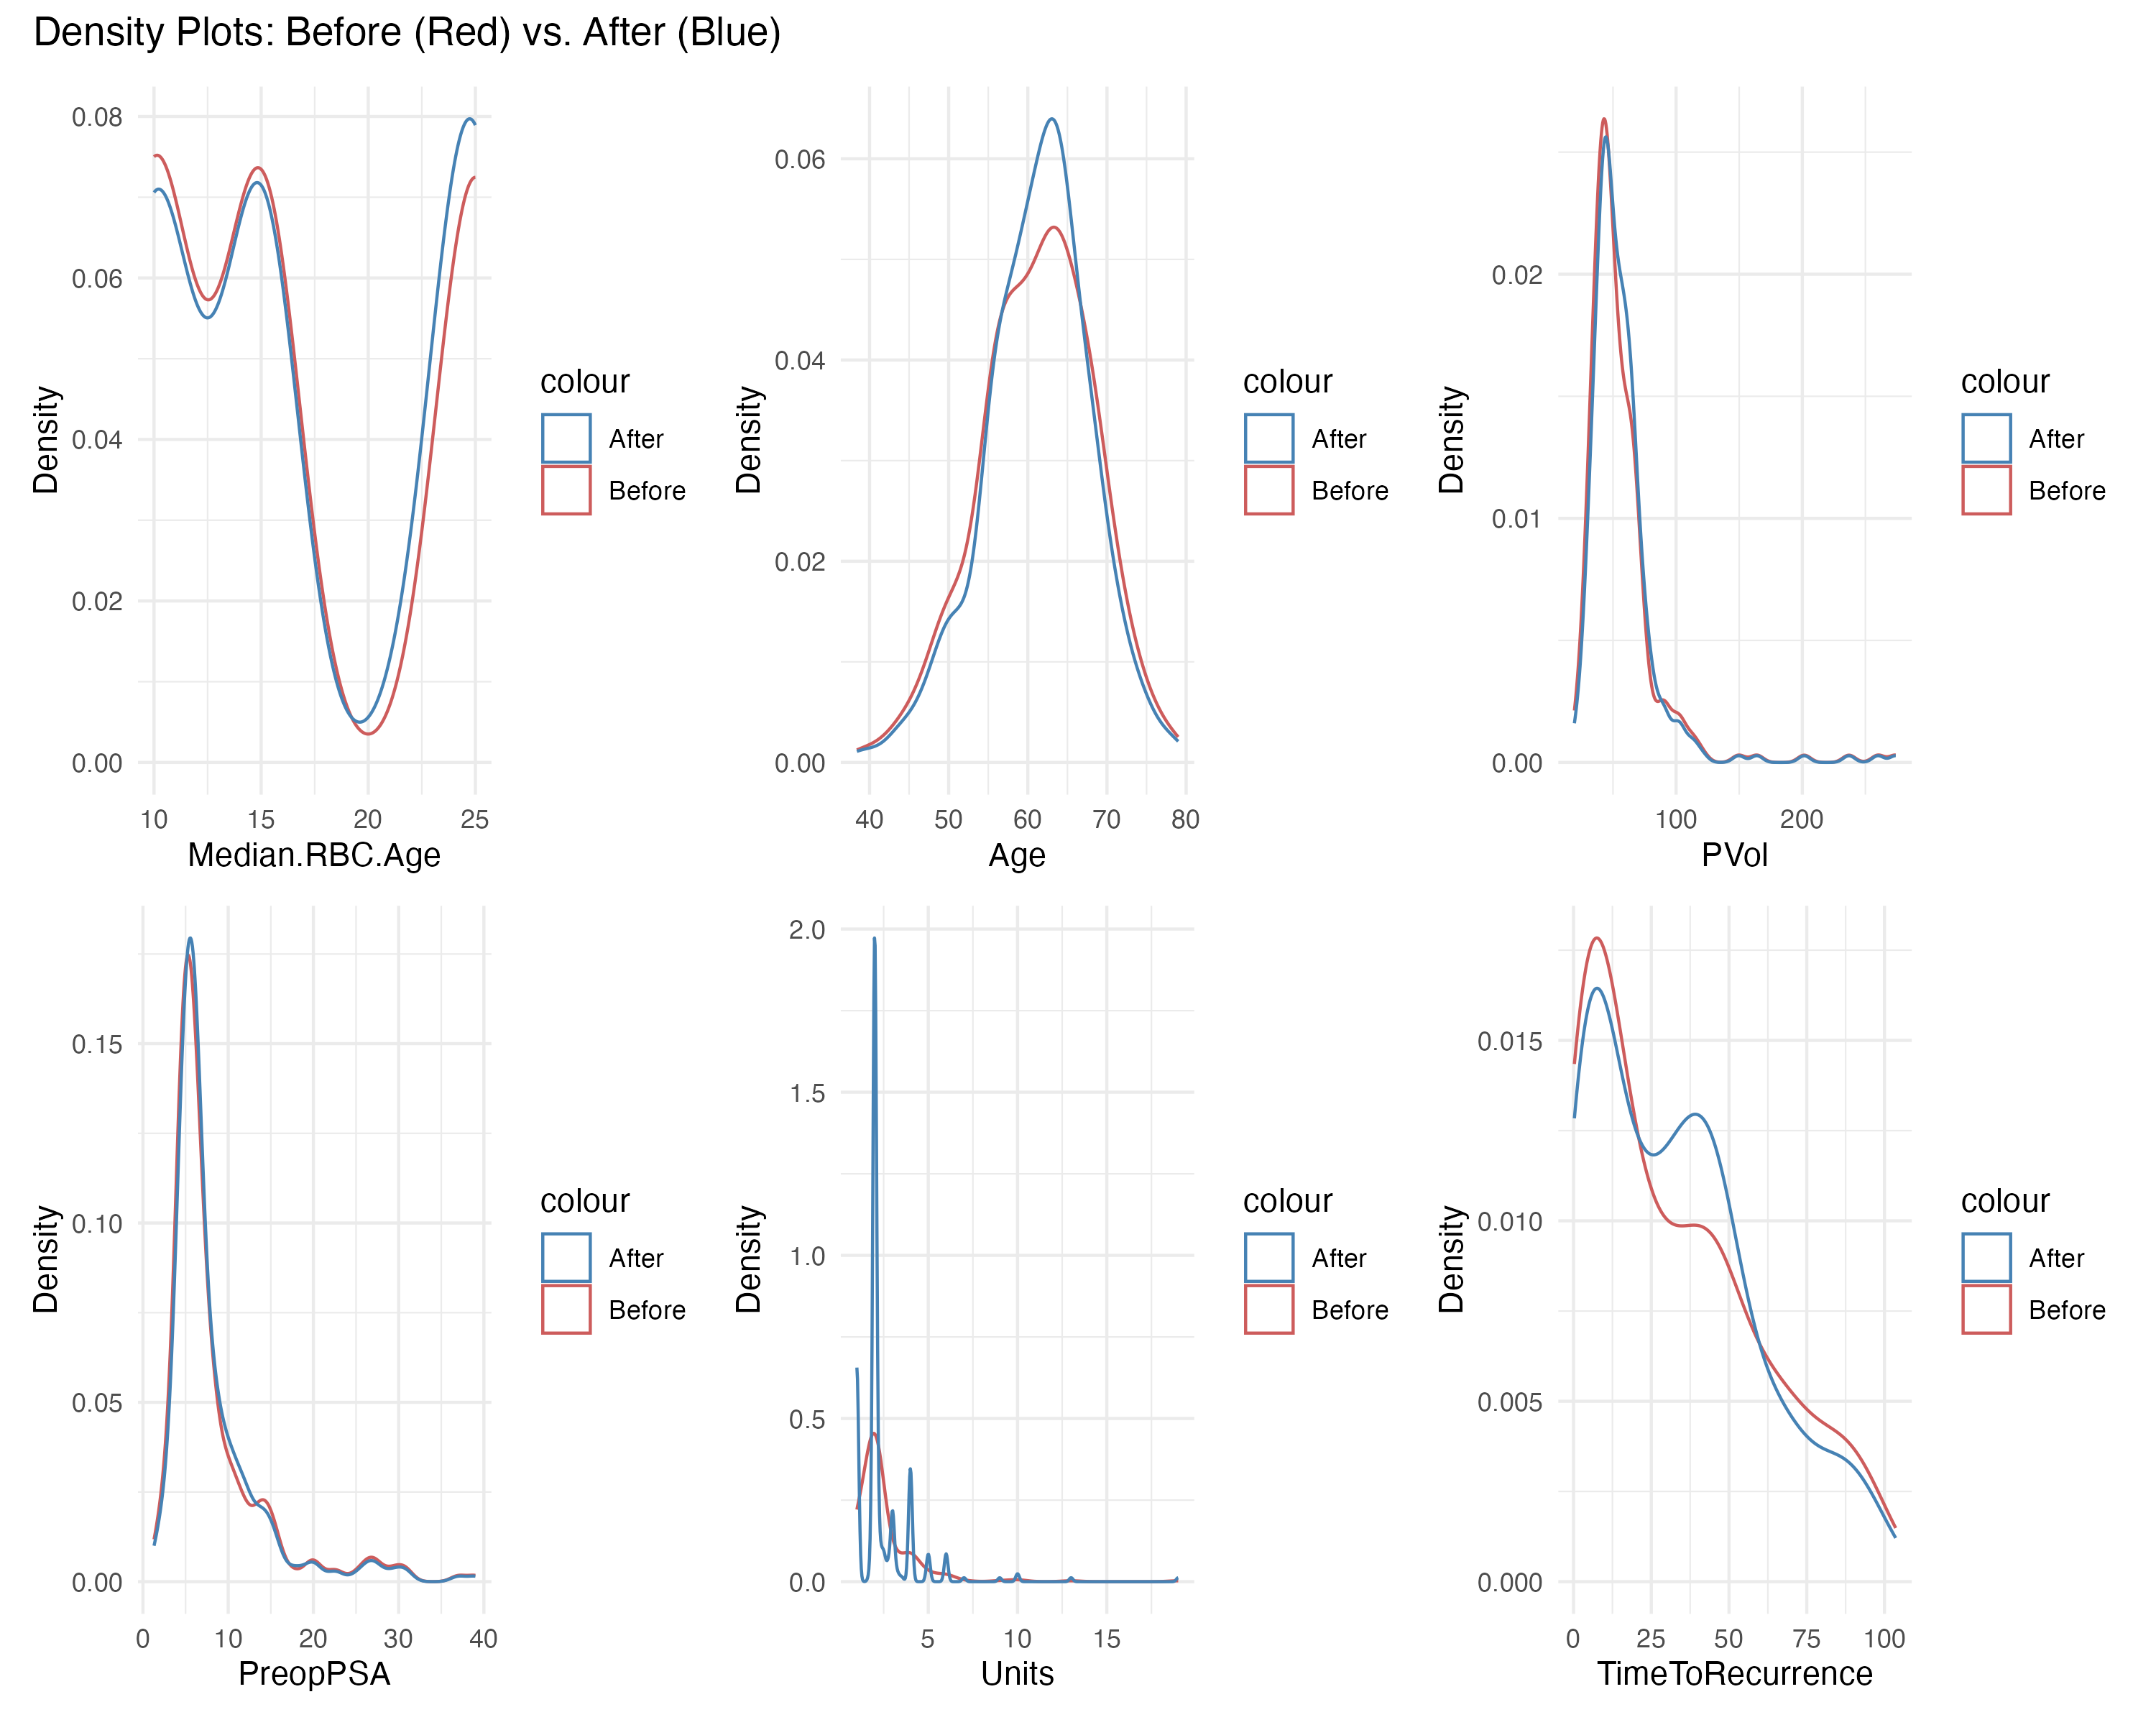
\includegraphics[width=0.9\linewidth]{../example/density_plots_before_after} 

}

\caption{Density Plots (Before vs After)}\label{fig:show-densityplot}
\end{figure}

\begin{figure}[H]

{\centering 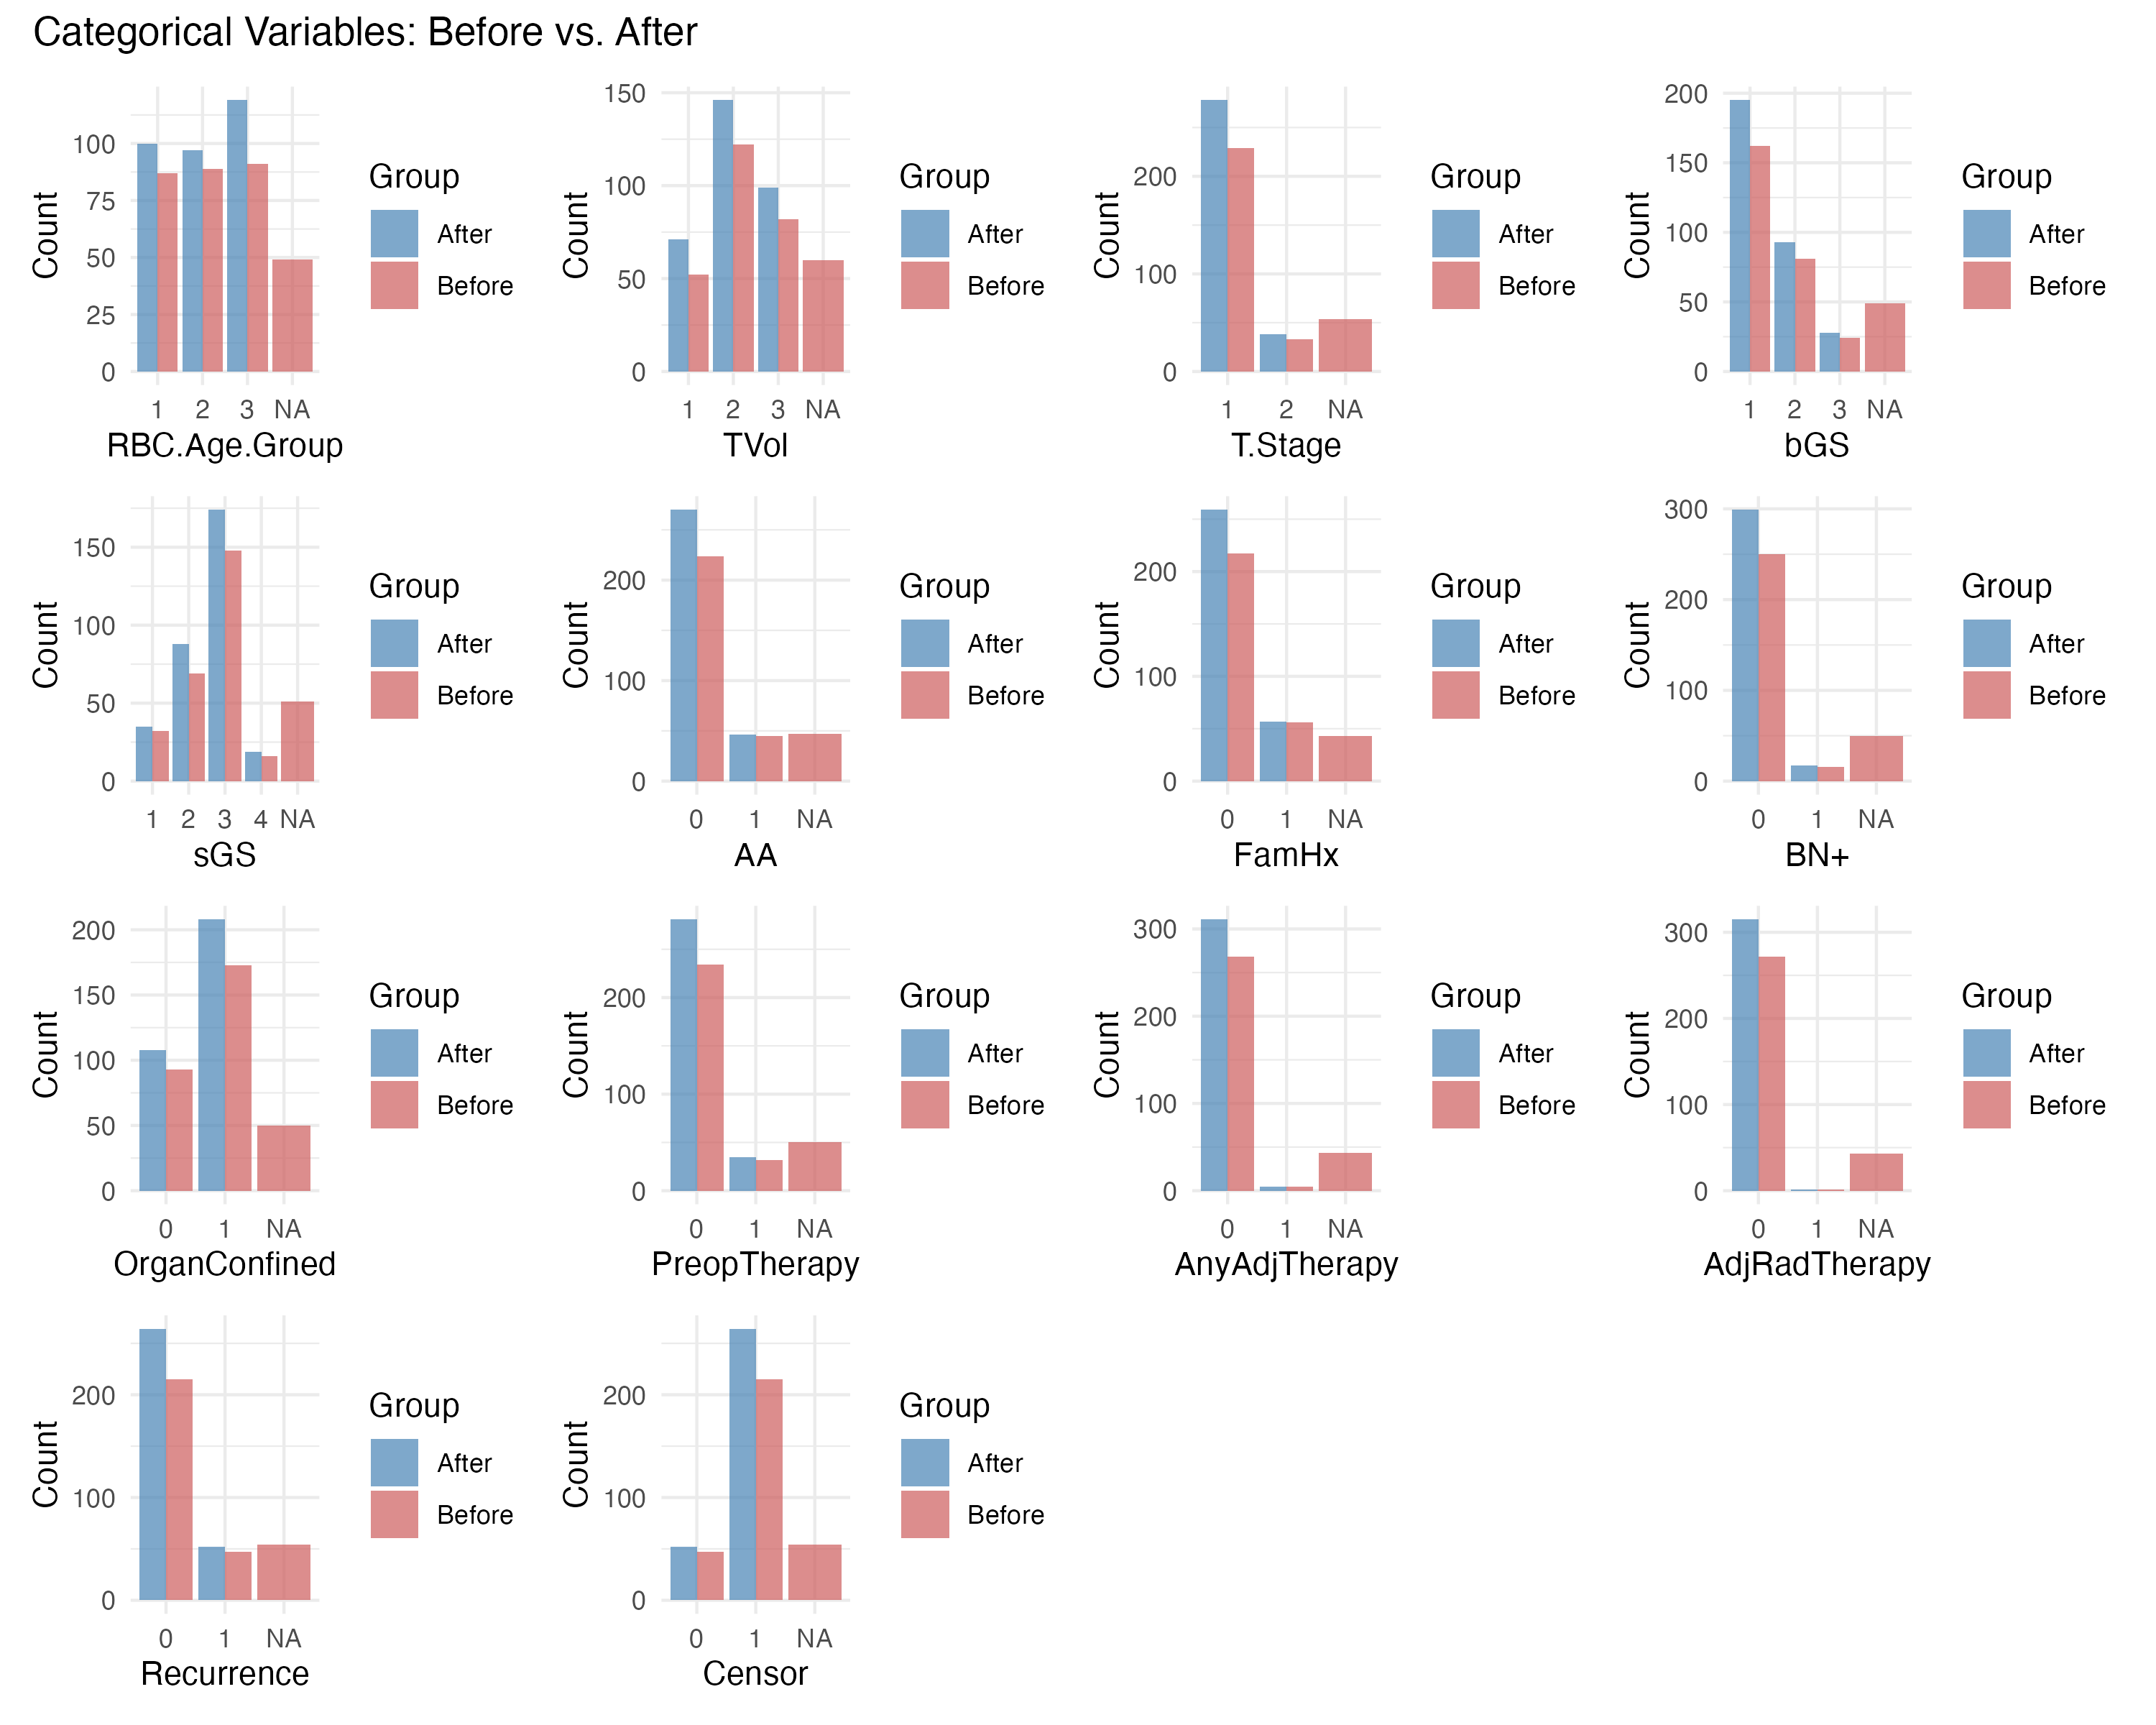
\includegraphics[width=0.9\linewidth]{../example/barplots_cat_before_after} 

}

\caption{Bar Plots (Before vs After)}\label{fig:show-barplot}
\end{figure}

\section{Interpretation Guide}\label{interpretation-guide}

\begin{itemize}
\tightlist
\item
  \textbf{Correlation Heatmaps}: Red/blue tiles indicate strong
  positive/negative correlations.
\item
  \textbf{Model Performance Table}: Compare methods (Random Forest, KNN,
  MICE, MiceForest) across missing rates using:

  \begin{itemize}
  \tightlist
  \item
    \textbf{Average MSE}: Lower is better for numeric variables.
  \item
    \textbf{Average Accuracy}: Higher is better for categorical
    variables.
  \item
    \textbf{Best K (KNN only)}: The value of \texttt{k} yielding best
    performance.
  \end{itemize}
\item
  \textbf{Imputation Comparison}: Boxplots and density plots illustrate
  that the distribution of imputed values aligns well with original
  patterns.
\item
  The imputation method with lowest MSE and high accuracy is applied to
  generate the final complete dataset.
\end{itemize}

\end{document}
